\documentclass{article}[12pt,a4paper]

%!TEX root = main.tex

\def\finex{{\unskip\nobreak\hfil
\penalty50\hskip1em\null\nobreak\hfil{\Large $\diamond$}
\parfillskip=0pt\finalhyphendemerits=0\endgraf}}

\newenvironment{lmref}[1]{%
	\vspace*{0.3cm}
	\noindent {\bf  Lemma #1.}}

\newenvironment{thref}[1]{%
	\vspace*{0.3cm}
	\noindent {\bf  Theorem #1.}}

\newenvironment{corref}[1]{%
	\vspace*{0.3cm}
	\noindent {\bf  Corollary #1.}}


\newcommand{\picalc}{$\pi$-calculus~}
\newcommand{\ms}[1]{\mathsf{#1}}
\newcommand{\ctx}{\mathtt{C}}
\newcommand{\co}[1]{\overline{#1}}
\newcommand{\proj}[1]{\mathtt{proj}(#1)}
\newcommand{\projs}[1]{\mathtt{proj_n}(#1)}
\newcommand{\lts}[1]{\xrightarrow{#1}}
\newcommand{\comm}[1]{\textcolor{blue}{#1}}
\newcommand{\red}[1]{\textcolor{red}{#1}}
\newcommand{\key}{\mathtt{keys}}
\newcommand{\flts}[1]{\overset{#1}\twoheadrightarrow}
\newcommand{\rev}{^{\bullet}}
%\newcommand{\forw}{_{\twoheadrightarrow}}
\newcommand{\eq}{\sim} 
\newcommand{\env}{\theta} 
\newcommand{\ex}{e} 
\newcommand{\proc}[3]{\langle #1,#2,#3\rangle } 
\newcommand{\erl}[1]{\hookrightarrow_{#1}} 
\newcommand{\mem}[2]{[#1\;;#2]}
\newcommand{\bl}[1]{\textcolor{blue}{#1}}
\newcommand{\rd}[1]{\textcolor{red}{#1}}
\newcommand{\mtt}[1]{\mathtt{#1}}
\newcommand{\pid}{\mathtt{pid}}
\newcommand{\procl}[4]{\langle #1,#2,#3,#4\rangle } 
\newcommand{\con}{\equiv}
\newcommand{\conk}{\equiv_k}
\newcommand{\extcon}{\equiv_c}
\newcommand{\de}{\delta}
\newcommand{\G}{\Gamma}
\newcommand{\logg}[1]{\rightharpoonup_{#1}}
\newcommand{\rlogg}[1]{\leftharpoondown_{#1}}
\newcommand{\la}{\lambda}
\newcommand{\col}[1]{\mathtt{col}(#1)}
\newcommand{\rel}{\mathcal{R}}
\newcommand{\conc}{\smile_c}
\newcommand{\nil}{{\bf{0}}}
%\newcommand{\res}{\nu}
\newcommand{\res}[1]{\nu #1\,}
\newcommand{\out}[1]{\langle #1\rangle}
\newcommand{\cont}{\triangleright}
\newcommand{\sub}[2]{\{#1/#2\}}
\newcommand{\op}{op_n}
\newcommand{\pidd}{Pid}
\newcommand{\fmod}{\rightarrowtail}
\newcommand{\enc}[1]{\llparenthesis #1 \rrparenthesis}
\newcommand{\blt}{\bullet}
\newcommand{\str}{C}
\newcommand{\term}[1]{T[#1]}
\newcommand{\en}[1]{\Lbag #1 \Rbag}
\newcommand{\signal}[1]{\{ #1\}}
\newcommand{\systset}{\mathbb{S}}
\newcommand{\confset}{\mathbb{C}}
\newcommand{\set}[1]{\{ #1\}}
\newcommand{\node}[3]{#1,#2\mkern-3mu:\mkern-3mu[\mkern-6mu[#3]\mkern-6.2mu]}


\usepackage{listings}
\usepackage[version=3]{mhchem} % Package for chemical equation typesetting
\usepackage{siunitx} % Provides the \SI{}{} and \si{} command for typesetting SI
\usepackage{algorithm}
\usepackage{algpseudocode}
% units
\usepackage{fancyvrb}
\usepackage{hyperref}
\usepackage{breakurl}             % Not needed if you use pdflatex only.
\usepackage{underscore}           % Only needed if you use pdflatex.
\usepackage{microtype}%if unwanted, comment out or use option "draft"
\usepackage{amssymb}
\usepackage{cleveref}
\setcounter{tocdepth}{3}
\usepackage{graphicx}
\usepackage{listings}
\usepackage{color}
\usepackage{rotating}
\usepackage{todonotes}
\usepackage{mathpartir}
\usepackage{url}
\usepackage{tikz}
\usepackage{amsmath}
\usepackage{stmaryrd}
\usepackage{amsthm}
\usepackage{float}
\usepackage{hyperref}
\usepackage{thm-restate}

\usetikzlibrary{matrix}

\renewcommand{\labelenumi}{\alph{enumi}.} % Make numbering in the enumerate environment by letter rather than number (e.g. section 6)

\theoremstyle{definition}
\newtheorem{example}{Example}[section]
\newtheorem{theorem}{Theorem}

\newtheorem{case}{Case}

\newtheorem{definition}{Definition}
\newtheorem{lemma}{Lemma}
\newcommand{\paral}{\;|\;}
\newcommand{\cons}{\mbox{:}}

\begin{document}

\section{Consistency}

\begin{figure}
  \centering
  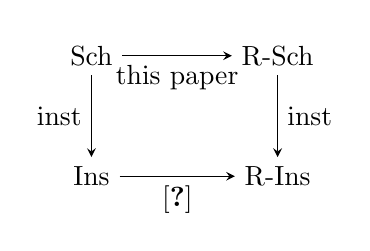
\begin{tikzpicture}
    \centering \matrix (m) [matrix of math nodes,row sep=3em,column
    sep=4em,minimum width=2em] {
      \text{Sch} & \text{R-Sch} \\
      \text{Ins} & \text{R-Ins} \\}; \path[-stealth] (m-1-1) edge node [left]
    {inst} (m-2-1) edge node [below] {this paper} (m-1-2)
    (m-2-1.east|-m-2-2) edge node [below] {\cite{LaneseM20}} node [] {} (m-2-2)
    (m-1-2) edge node [right] {inst} (m-2-2);
  \end{tikzpicture}
  \caption{ Schema of the proof of correctness. }
  \label{fig:square}
\end{figure}

In Fig.~\ref{fig:square} we can observe the relation occurring between schemas
and instances. On the top-left corner we have non-reversible schemas, on the
top-right we have reversible schemas, while below on the
bottom-right corner we have concrete non-reversible instances - i.e., ground
rules - and on the bottom-left corner we have concrete reversible instances.

Schemas differ from instances as they admit the presence of meta-variables that
can range over ground terms. Intuitively, to get from one of the top corners to
the respective concrete one we need to instantiate each meta-variable with
the appropriate ground instance. The correctness of the rule is then ensured by
the set of equations each rule is equipped with, if the concrete instances of
the meta-variables satisfy the equational condition then the instance of the
rule is to be considered correct.\\

Now, let us discuss the top-arrow, that is transforming a non-reversible schema in reversible
schema. A non-reversible schema has the following shape:
\[t \rightarrow t'~\ms{if}~\overline{eq}_n\]
where $t$ and $t'$ are inductively defined as
\[
  \begin{array}{l}
    t,t',t_1,\ldots,t_n: ::=\\
    \hspace{1ex}|~e\\
    \hspace{1ex}|~op(t_1,\ldots,t_n)\\
  \end{array}
\]

Now, for a schema to be reversible each entity must be tagged with a unique meta-key and a
memory has to be produced each time that a transition is performed. In symbols
\[t_r \rightarrow t'_r \paral \mu ~\ms{if}~\overline{eq}_n~\text{where
  }ukeys(t_r\rightarrow t'_r)\]

Where $t_r$ and $t'_r$ are inductively defined as
\[
  \begin{array}{l}
    t_r,t'_r,t_{1r},\ldots,t_{nr} ::=\\
    \hspace{1ex}|~e*k\\
    \hspace{1ex}|~op(t_{1r},\ldots,t_{nr})\\
  \end{array}
\]
and $\mu$ is defined as $[R;C]$ where $R$ is the configuration that gave rise to
the step, i.e., $t_r$, and $C$ is a context describing the structure of the
resulting one, where entities have been removed and replaced with a hole $\bullet$, while keys are kept.

In symbols $C$ is inductively defined as
\[
  \begin{array}{l}
    c,c',c_1,\ldots,c_n ::=\\
    \hspace{1ex}|~\bullet*k\\
    \hspace{1ex}|~op(c_1,\ldots,c_n)\\
  \end{array}
\]
  
Let us define the $tag$ operation

\[
  \begin{array}{l}
    \begin{array}{l}
      tag(t\rightarrow t') ::=\\
      \hspace{2ex}\ms{let} (t_r, keys) = tag\_left(t, K)~\ms{in}\\
      \hspace{2ex}\ms{let} (t_r',\_,\_) = tag\_right(t', keys, 0)~\ms{in}\\
      \hspace{4ex}t_r \rightarrow t'_r
    \end{array}\\

  \begin{array}{l}
    tag\_left(t, k :: keys) ::=\\
    \hspace{2ex}\ms{match}~t~\ms{with}\\
    \hspace{4ex}| e \rightarrow (e*k',k'::k::keys)\\
    \hspace{4ex}| op(tlist) \rightarrow \\
    \hspace{6ex} \ms{let}~f=\ms{fun}(x,(rtlist, keys')) \rightarrow \ms{let}(x_r,keys'')=tag\_left(x, keys')~\ms{in}~(rtlist::x_r, keys'')~\ms{end}~\ms{in}\\
    \hspace{6ex} \ms{let}~(rtlist, keys') = \ms{foldl}~tlist~([],keys)~f~\ms{in}\\
    \hspace{8ex} (op(rtlist), keys')
  \end{array}\\

  \begin{array}{l}
    tag\_right(t, keys, c) ::=\\
    \hspace{2ex}\ms{match}~t~\ms{with}\\
    \hspace{4ex}| e \rightarrow \ms{let}~c'=c+1~\ms{in}\\
    \hspace{6ex} (e*c'::keys,c')\\
    \hspace{4ex}| op(tlist) \rightarrow \\
    \hspace{6ex} \ms{let}~f = (x,(rtlist,C,keys))\rightarrow \ms{let}(x_r,C')=tag\_right(x, keys, C)~\ms{in}~(rtlist::x_r,C', keys)~\ms{end}~\ms{in}\\
    \hspace{6ex} \ms{let}~(rtlist, C, keys') = \ms{foldl}~tlist~([],c,keys)~f~\ms{in}\\
    \hspace{8ex} (op(rtlist), C, keys')    
  \end{array}
  \end{array}
\]

The function $tag$ takes in input a non reversible schema and produces a
tagged version of the schema, where each entity is tagged with a unique meta-key. The meta-keys used to tag the
entities must be unique since then in the concrete instances each entity has to
be tagged with a unique concrete key, if in the schema two (or more) entities
would be tagged with the same meta-key then it would be impossible to
instantiate them to different values.

In order to simplify the proof of the correctness of the transformation instead
of the function $tag$ we will use relation $\rightsquigarrow_k$ to abstract the
transformation of terms. Relation $\rightsquigarrow_k$ is the least relation that
satisfies the following rules.

\[
  \begin{array}{ll}
    \displaystyle
    \frac{\ms{lw}(e)~~k\text{ is fresh}}
    { e \rightsquigarrow_k e * k }
    &
      \displaystyle
      \frac{t_1 \rightsquigarrow_k t'_1~\ldots~t_n\rightsquigarrow_k t'_n}
      { op[t_1,\ldots,t_n] \rightsquigarrow_k op[t'_1,\ldots,t'_n] }
  \end{array}
\]

Relation $\rightsquigarrow_k$ faithfully describes the behavior of both $tag\_right$
and $tag\_left$ as the rule on the left corresponds to the base case, where a
fresh key is attached to an entity of the lower level and the rule on the right
corresponds to the recursive call on the terms used by operator $op$. The
predicate $\ms{lw}$ makes sure that $e$ belongs to the lower level of the semantics.

Once a non-reversible schema has been tagged we need to produce the memory, for
that we rely on the function $mem$, that given a rule returns the rule together
with the appropriate memory.
\[
  \begin{array}{l}
  \begin{array}{l}
    mem(t_r \rightarrow t'_r) ::=\\
    \hspace{2ex}\ms{let}~C=ctx(t'_r)~\ms{in}\\
    \hspace{2ex}t_r \rightarrow t'_r~|~[C;t_r]
  \end{array}\\[5ex]
  
  \begin{array}{l}
    ctx(t)::=\\
    \hspace{2ex}\ms{match}~t~\ms{with}\\
    \hspace{4ex}| e*k \rightarrow \bullet * k\\
    \hspace{4ex}| op(\overline{t_r}) \rightarrow \\
    \hspace{6ex} \ms{let}~f=\ms{fun}(x,\overline{c_m})\rightarrow~\overline{c_m}::ctx(x)~\ms{end}~\ms{in}\\
    \hspace{6ex}\ms{let}~\overline{c_n} =
    \ms{foldl}~(\overline{t_r})~[\:]~f~\ms{in}\\
    \hspace{8ex} op(\overline{c_n})
  \end{array}
  \end{array}
\]

To abstract function $ctx$ we rely on the least relation that satisfies
$\rightsquigarrow_h$.

\[
  \begin{array}{ll}
    \displaystyle
    \frac{}
    { e * k \rightsquigarrow_h \bullet * k }
    &
      \displaystyle
      \frac{t_1 \rightsquigarrow_h t'_1~\ldots~t_n\rightsquigarrow_h t'_n}
      { op[t_1,\ldots,t_n] \rightsquigarrow_h op[t'_1,\ldots,t'_n] }
  \end{array}
\]

Now we can define the transformation of a non-reversible rule $t\rightarrow t'$
to (one of) its reversible counterparts $t_r \rightsquigarrow t'_r|\mu$ in terms of
$\rightsquigarrow$.

\[
  \frac{t\rightsquigarrow_k t_r~~~~t'\rightsquigarrow_k t'_r~~~~t'_r\rightsquigarrow_h ctx}{
    t\rightarrow t'~\ms{if}~C \rightsquigarrow t_r \rightarrow t'_r|[ctx; t_r]~\ms{if}~C 
  }
\]

Now, for the transformation to be correct two ingredients are needed: i) that
each entity is tagged with a unique meta-key and ii) that the context produced
is correct in the sense that each entity of the right-hand side reversible term
has been replaced by a hole.

\begin{lemma}[Unicity of keys]\label{lemma:keys}
  Relation $\rightsquigarrow_k$ tags each entity of a term $t$ with a unique key.
\end{lemma}
\begin{proof}
  We proceed by induction on the structure of $t$.\\
  Case $t = e$.\\
  The case of single entity is easy as the entity is left
  untouched and tagged with a fresh key.\\
  Case $t = op[t_1,\ldots,t_n]$.\\
  By inductive hypothesis we know that entities inside each $t'_i$ have been already tagged with
  fresh keys, where $t_i\rightsquigarrow_k t'_i$ for $1 \leq i \leq n$, so we can
  conclude that $op[t'_1,\ldots,t'_n]$ is tagged with unique keys.
\end{proof}

\begin{lemma}[Correctness of Context]\label{lemma:ctx}
  Relation $\rightsquigarrow_h$, given a term $t$, produces the correct context,
  that is the same system where all the entities have been replaced by a hole $\bullet$.
\end{lemma}
\begin{proof}
  We proceed by induction on the structure of $t$.\\
  Case $t = e$.\\
  The case of single entity is easy as the entity is replaced with a hole and
  the key left untouched.\\
  Case $t = op[t_1,\ldots,t_n]$.\\
  By inductive hypothesis we know that each $t'_i$ has been already transformed
  and entities have been replaced by holes, where $t_i\rightsquigarrow_k t'_i$ for $1 \leq i \leq n$, so we can
  conclude that $op[t'_1,\ldots,t'_n]$ is the correct context.
\end{proof}

By \cref{lemma:keys,lemma:ctx} we can conclude that $\rightsquigarrow$ is
a correct transformation. 

\section{From Schemas to Ground Rules}

The last part to show is that our schemas can be instantiated to the format
expected by the general approach. To achieve so we rely on an instantiation
relation that replaces the variables present in the schemas with concrete values.

Before showing the instantiation we recall that in Maude a rule has the generic
following shape:
\[t \rightarrow t'~\ms{if}~C\]
and that the variables used in the rule are not exclusively only the variables
introduced in $t$ but that new variables can be introduced in $C$ as well.

We define the instantiation of a schema to a ground rule in terms of the least
relation that satisfies the set of rules depicted in Fig.~\ref{fig:inst}.

\begin{figure}
  \centering
  $
  \begin{array}{c}
  \begin{array}{ll}
      \displaystyle
      \frac{replace(r,v,c_v),\mathcal{I}\rightarrow_I r'}
      {r, \{(v,c_v)\}\cup\mathcal{I} \rightarrow_I r'}
    &
      \displaystyle
      \frac{var(lhs(r))=\emptyset}
      {r,\emptyset \rightarrow_I r}
  \end{array}\\[5ex]

  \begin{array}{c}
    \displaystyle
    \frac{r,\mathcal{I}\rightarrow_I r'~~~E\vdash r'=t\rightarrow t'~\ms{if}~C}
    {r, \mathcal{I},E \rightsquigarrow t\rightarrow t'}
  \end{array}
  \end{array}
  $
  \caption{Instantiation relation}
  \label{fig:inst}
\end{figure}

Relation $\rightarrow_I$ is the relation that replaces variable inside a rule,
when all the variables have been replaced the bottom case is reached. Relation
$\rightsquigarrow$ relies on relation $\rightarrow_I$ to get a version of rule $r$
where all the vars of the rule have been substituted with concrete values,
except for the ones declared in the conditional branch.

The set $\mathcal{I}$ is assumed to be built as follow:
\[\mathcal{I}=\{(v,c_v)|v\in var(lhs(r)), sort(c_v)= sort(v)\}\]

Here, $var$ returns the set of variables used inside a term, $lhs$ returns
the left-hand side term of a rule and $sort$ the sort of the variable fed as
input.
We also assume that each rule is equipped with a conditional branch, where in
the case of unconditional rules - like the backward rules - we assume them to be
equipped with a dummy condition, like $true = true$.

Finally, when all the
variables, introduced in the left-hand side term, have been replaced everywhere the rule is brought to a canonical form, by relying on the
equations of the rewriting logic ($E\vdash r = t\rightarrow t'~\ms{if}~C$).

Let us make this more concrete with an example.
\begin{example}
  Let us consider the meta-rule \verb+tau+ and the equation about matching.
\begin{Verbatim}
  crl [sys-tau] :
      < P | exp: EXSEQ, env-stack: ENV, ASET >  =>
      < P | exp: EXSEQ', env-stack: ENV', ASET >
      if < tau, ENV', EXSEQ' > :=
         < req-gen, ENV, EXSEQ > .

  eq [match] :
   < REQLABEL, ENVSTACK, GVALUE = GVALUE > =
   < tau, ENVSTACK, GVALUE > .

\end{Verbatim}

  Then let us consider the following $\mathcal{I}$:
  \[\{(\verb+EXSEQ+,\verb+true = true+),(\verb+P+,\verb+2+), (\verb+ENV+, \verb+{}+)\}\]
\end{example}

For the sake of simplicity we will ignore the components of a process inside
\verb+ASET+ as they are not relevant for this example (\verb+ASET+ currently
only contains the definitions of the functions that the process is allowed to
invoke).

Now, after substituting the variables with their current values we obtain a rule
with the following shape.

\begin{Verbatim}
  crl [sys-tau] :
      < 2 | exp: true = true, env-stack: {}, _ >  =>
      < 2 | exp: EXSEQ', env-stack: ENV', _ >
      if < tau, ENV', EXSEQ' > :=
         < req-gen, {}, true = true > .
\end{Verbatim}

Then, the only equation that can be applied is equation \verb+match+ depicted
above and after its application the rule will have the following shape.

\begin{Verbatim}
  crl [sys-tau] :
      < 2 | exp: true = true, env-stack: {}, _ >  =>
      < 2 | exp: true, env-stack: {}, _ >
      if < tau, {}, true > :=
         < req-gen, {}, true = true > .
\end{Verbatim}

Finally, since we have instantiated all the variables with ground values and
verified the conditional branch with the equational theory we can drop it and
obtain a concrete rule that fits the format required by the general approach.

\begin{Verbatim}
      < 2 | exp: true = true, env-stack: {}, _ >  =>
      < 2 | exp: true, env-stack: {}, _ >
\end{Verbatim}

\subsection{Remark About Keys}

This subsection contains a remark about the handling of keys in schemas and in
the ground rules. In the general methods keys are picked up fresh to tag each
ground entity and there are no other constraints on the choice of keys. In our
approach, since we need an operational way to apply the schemas to concrete
system instances, we need to
specify concretely in which way we pick the meta-keys. The method adopted
consists of using a set of meta-keys while tagging the left-hand side of a rule
and concatenating the first meta-key used on the left-hand side with a fresh
counter for the entities on the right.

The technique used to tag the right-hand side of the rule, since it concatenates
a ground value with a meta-key, prevents us to instantiate the meta-keys on the
left to arbitrary values as their prefix has been already chosen. In other
words, the set of ground rules is a subset of the entirety of the rules produced
by the general method. Nonetheless, this is not a limit as all the possible
transitions of a system can still be expressed, only there is an order on the way
keys are picked. So, up to keys permutation, the derived semantics is ``complete''.

\end{document}
